\documentclass[11pt,a4paper]{report}
\usepackage[textwidth=37em,vmargin=30mm]{geometry}
\usepackage{calc,xunicode,amsmath,amssymb,paralist,enumitem,tabu,booktabs,datetime2,xeCJK,xeCJKfntef,listings}
\usepackage{tocloft,fancyhdr,tcolorbox,xcolor,graphicx,eso-pic,xltxtra,xelatexemoji}

\newcommand{\envyear}[0]{2024}
\newcommand{\envdatestr}[0]{2024-11-02}
\newcommand{\envfinaldir}[0]{webdb/2024/20241102/final}

\usepackage[hidelinks]{hyperref}
\hypersetup{
    colorlinks=false,
    pdfpagemode=FullScreen,
    pdftitle={Web Digest - \envdatestr}
}

\setlength{\cftbeforechapskip}{10pt}
\renewcommand{\cftchapfont}{\rmfamily\bfseries\large\raggedright}
\setlength{\cftbeforesecskip}{2pt}
\renewcommand{\cftsecfont}{\sffamily\small\raggedright}

\setdefaultleftmargin{2em}{2em}{1em}{1em}{1em}{1em}

\usepackage{xeCJK,xeCJKfntef}
\xeCJKsetup{PunctStyle=plain,RubberPunctSkip=false,CJKglue=\strut\hskip 0pt plus 0.1em minus 0.05em,CJKecglue=\strut\hskip 0.22em plus 0.2em}
\XeTeXlinebreaklocale "zh"
\XeTeXlinebreakskip = 0pt


\setmainfont{Brygada 1918}
\setromanfont{Brygada 1918}
\setsansfont{IBM Plex Sans}
\setmonofont{JetBrains Mono NL}
\setCJKmainfont{Noto Serif CJK SC}
\setCJKromanfont{Noto Serif CJK SC}
\setCJKsansfont{Noto Sans CJK SC}
\setCJKmonofont{Noto Sans CJK SC}

\setlength{\parindent}{0pt}
\setlength{\parskip}{8pt}
\linespread{1.15}

\lstset{
	basicstyle=\ttfamily\footnotesize,
	numbersep=5pt,
	backgroundcolor=\color{black!5},
	showspaces=false,
	showstringspaces=false,
	showtabs=false,
	tabsize=2,
	captionpos=b,
	breaklines=true,
	breakatwhitespace=true,
	breakautoindent=true,
	linewidth=\textwidth
}






\newcommand{\coverpic}[2]{
    % argv: itemurl, authorname
    Cover photo by #2~~(\href{#1}{#1})
}
\newcommand{\makeheader}[0]{
    \begin{titlepage}
        % \newgeometry{hmargin=15mm,tmargin=21mm,bmargin=12mm}
        \begin{center}
            
            \rmfamily\scshape
            \fontspec{BaskervilleF}
            \fontspec{Old Standard}
            \fontsize{59pt}{70pt}\selectfont
            WEB\hfill DIGEST
            
            \vfill
            % \vskip 30pt
            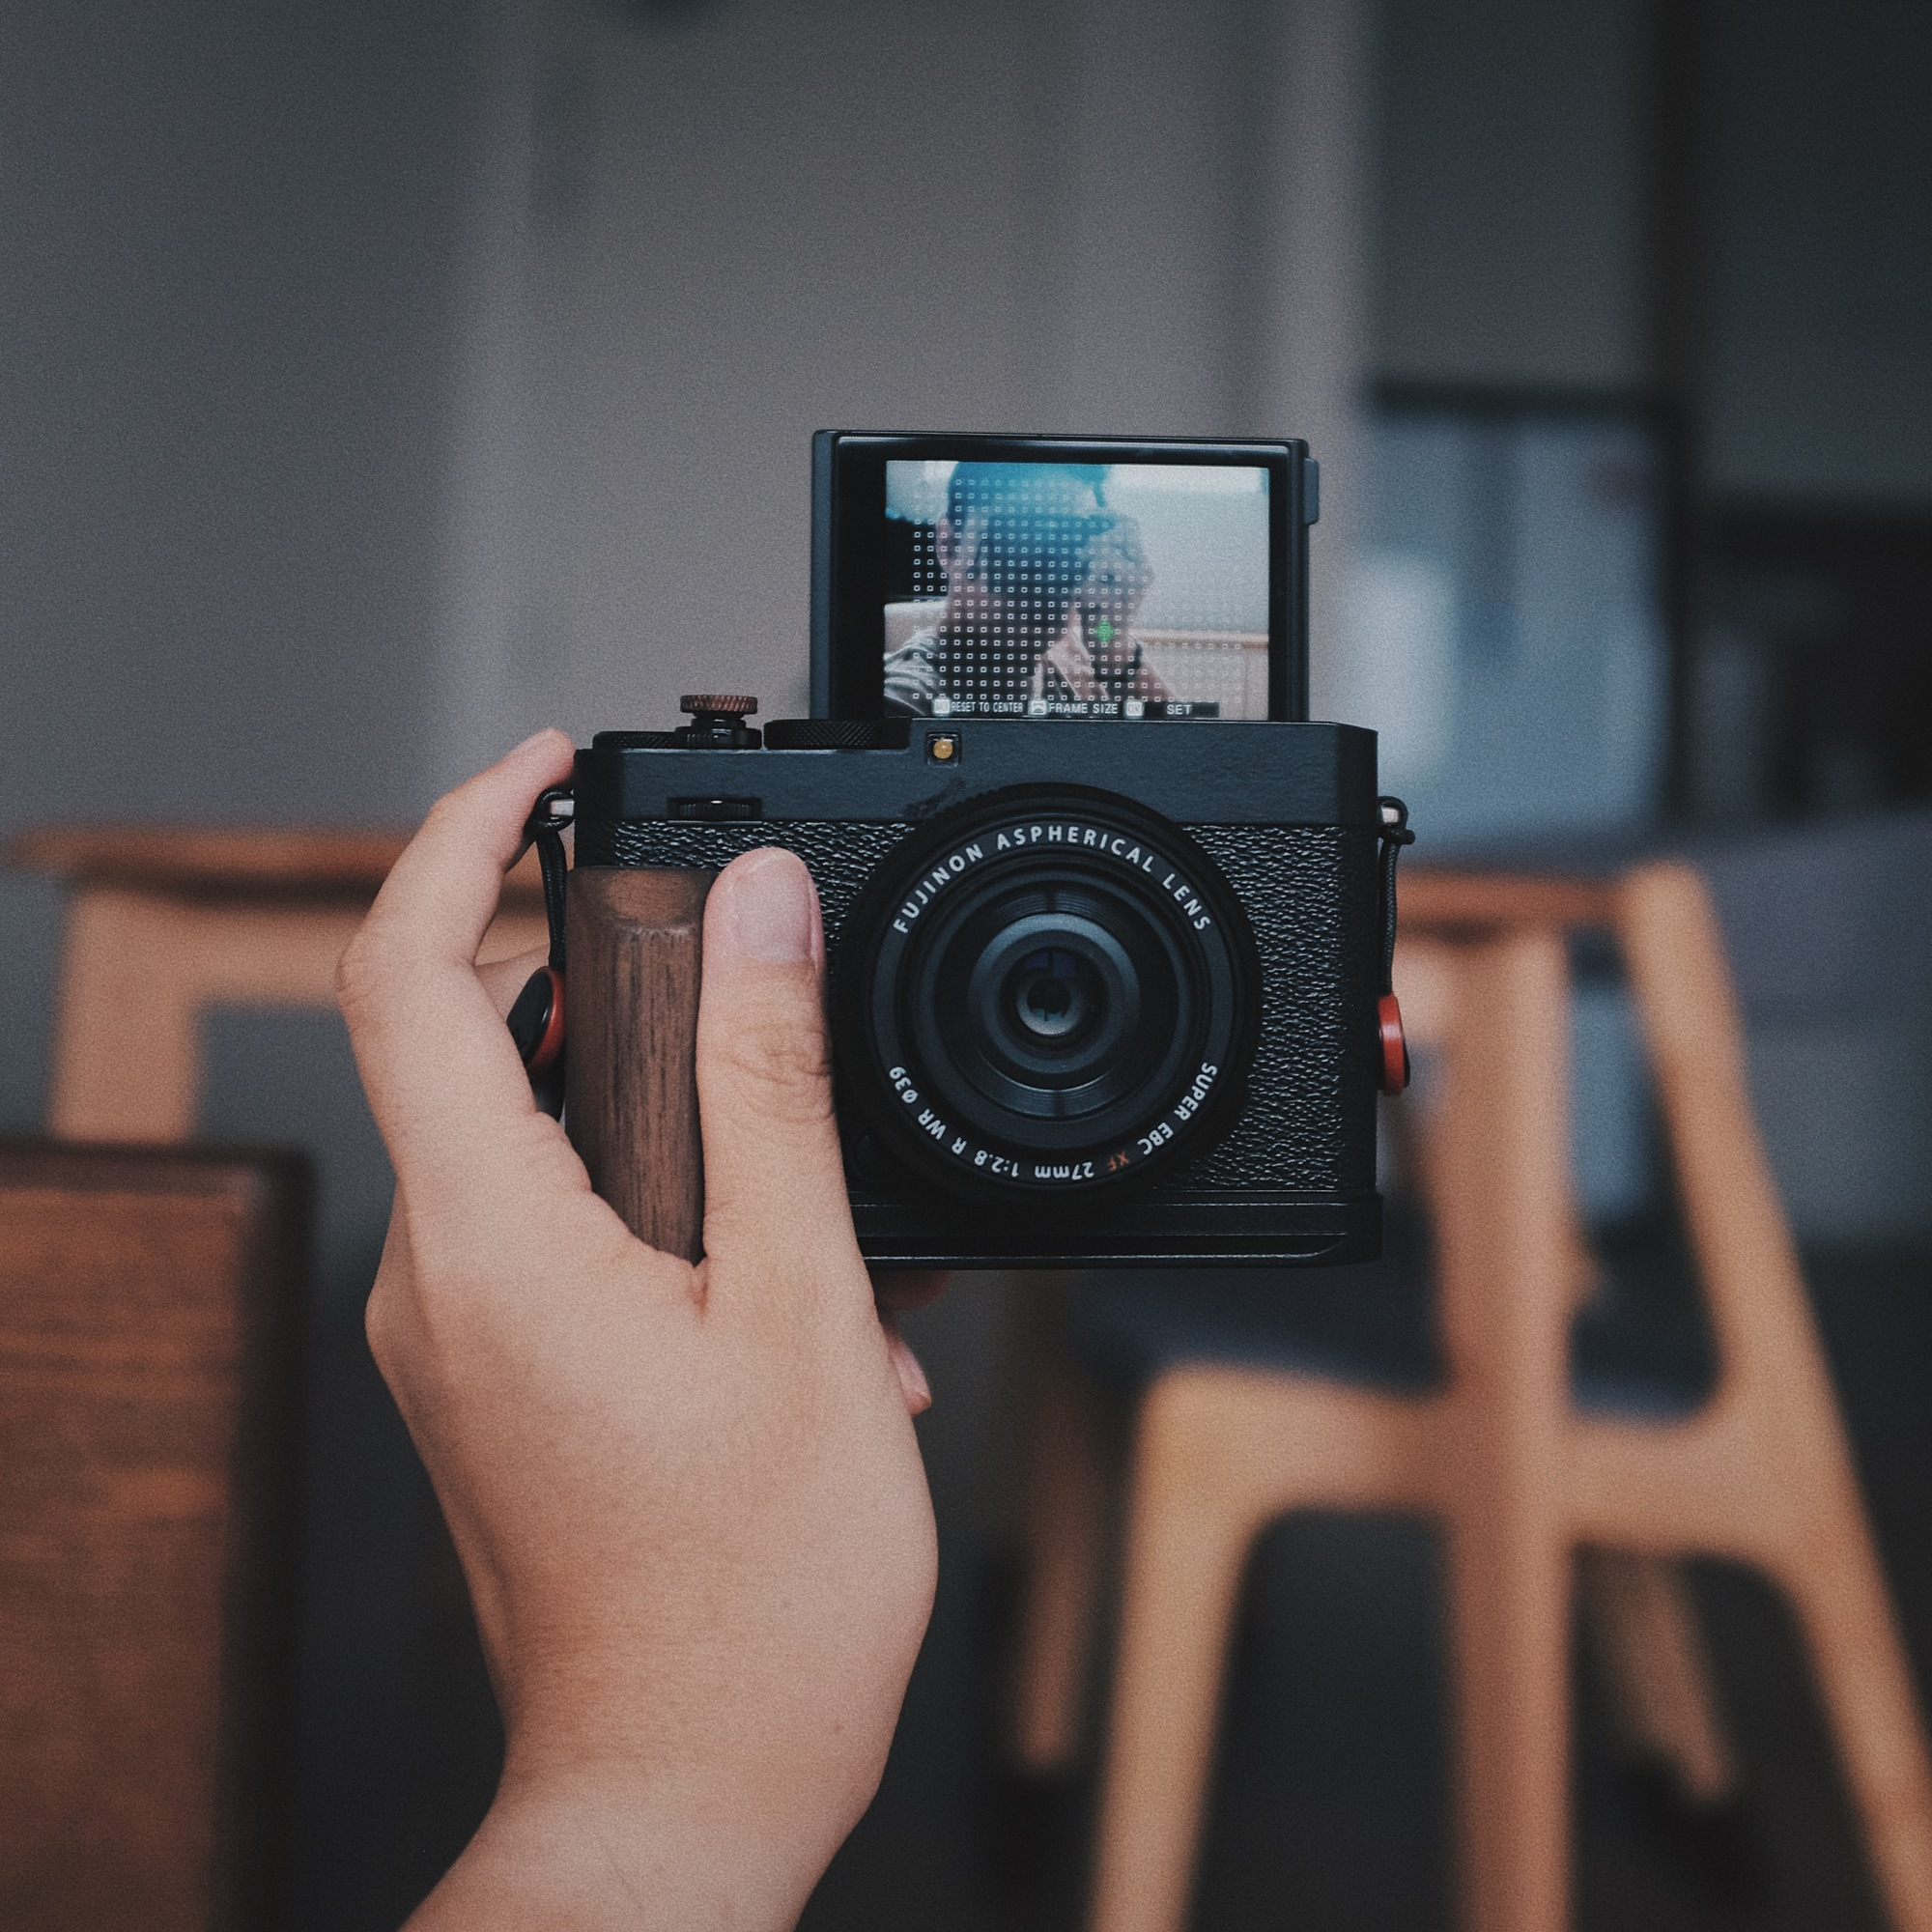
\includegraphics[width=\linewidth]{\envfinaldir/coverpic-prod.jpg}\par
            % \vskip 30pt
            \vfill

            \normalsize\rmfamily\scshape
            \copyright{} The Web Digest Project \hfill\large \envdatestr
        \end{center}
    \end{titlepage}
    % \restoregeometry
}
\newcommand{\simplehref}[1]{%
    \textcolor{blue!80!green}{\href{#1}{#1}}%
}
\renewcommand{\contentsname}{\center\Huge\sffamily\bfseries Contents\par\vskip 20pt}
\newcounter{ipartcounter}
\setcounter{ipartcounter}{0}
\newcommand{\ipart}[1]{
    % \vskip 20pt
    \clearpage
    \stepcounter{ipartcounter}
    \phantomsection
    \addcontentsline{toc}{chapter}{#1}
    % \begin{center}
    %     \Huge
    %     \sffamily\bfseries
    %     #1
    % \end{center}
    % \vskip 20pt plus 7pt
}
\newcounter{ichaptercounter}
\setcounter{ichaptercounter}{0}
\newcommand{\ichapter}[1]{
    % \vskip 20pt
    \clearpage
    \stepcounter{ichaptercounter}
    \phantomsection
    \addcontentsline{toc}{section}{\numberline{\arabic{ichaptercounter}}#1}
    \begin{center}
        \Huge
        \sffamily\bfseries
        #1
    \end{center}
    \vskip 20pt plus 7pt
}
\newcommand{\entrytitlefont}[1]{\subsection*{\raggedright\Large\sffamily\bfseries#1}}
\newcommand{\entryitemGeneric}[2]{
    % argv: title, url
    \parbox{\linewidth}{
        \entrytitlefont{#1}\par\vskip 5pt
        \footnotesize\ttfamily\mdseries
        \simplehref{#2}
    }\vskip 11pt plus 11pt minus 1pt
}
\newcommand{\entryitemGithub}[3]{
    % argv: title, url, desc
    \parbox{\linewidth}{
        \entrytitlefont{#1}\par\vskip 5pt
        \footnotesize\ttfamily\mdseries
        \simplehref{#2}\par\vskip 5pt
        \small\rmfamily\mdseries#3
    }\vskip 11pt plus 11pt minus 1pt
}
\newcommand{\entryitemAp}[3]{
    % argv: title, url, desc
    \parbox{\linewidth}{
        \entrytitlefont{#1}\par\vskip 5pt
        \footnotesize\ttfamily\mdseries
        \simplehref{#2}\par\vskip 5pt
        \small\rmfamily\mdseries#3
    }\vskip 11pt plus 11pt minus 1pt
}
\newcommand{\entryitemHackernews}[3]{
    % argv: title, hnurl, rawurl
    % \parbox{\linewidth}{
    %     \entrytitlefont{#1}\par\vskip 5pt
    %     \footnotesize\ttfamily\mdseries
    %     \simplehref{#3}\par
    %     \textcolor{black!50}{\href{#2}{#2}}
    % }\vskip 11pt plus 11pt minus 1pt
    \begin{minipage}{\linewidth}
            \entrytitlefont{#1}\par\vskip 5pt
            \footnotesize\ttfamily\mdseries
            \simplehref{#3}\par
            \textcolor{black!50}{\href{#2}{#2}}
    \end{minipage}\par\vskip 11pt plus 11pt minus 1pt
}







\begin{document}

\makeheader

\tableofcontents\clearpage




\ipart{Developers}
\ichapter{Hacker News}
\entryitemTwoLinks{Notepad++ is 21 years old}{https://news.ycombinator.com/item?id=42019586}{https://learnhub.top/celebrating-21-years-of-notepad-the-legendary-journey-of-our-favorite-text-editor/}

\entryitemTwoLinks{300 people applied to rent \$700/month sleeping pods in downtown San Francisco}{https://news.ycombinator.com/item?id=42019488}{https://www.theguardian.com/society/2024/oct/31/san-francisco-sleeping-pods-affordable-housing-crisis}

\entryitemTwoLinks{The rise of the U.S., the rise of China}{https://news.ycombinator.com/item?id=42018096}{https://www.construction-physics.com/p/how-china-is-like-the-19th-century}

\entryitemTwoLinks{Apple acquires Pixelmator}{https://news.ycombinator.com/item?id=42018013}{https://www.pixelmator.com/blog/2024/11/01/a-new-home-for-pixelmator/}

\entryitemTwoLinks{Ask HN: Who is hiring? (November 2024)}{https://news.ycombinator.com/item?id=42017580}{https://news.ycombinator.com/item?id=42017580}

\entryitemTwoLinks{Ask HN: Who wants to be hired? (November 2024)}{https://news.ycombinator.com/item?id=42017578}{https://news.ycombinator.com/item?id=42017578}

\entryitemTwoLinks{A new dental scam is to pull healthy teeth to sell you expensive fake ones}{https://news.ycombinator.com/item?id=42017428}{https://arstechnica.com/health/2024/11/more-dentists-are-pulling-healthy-teeth-to-sell-pricy-implants-experts-warn/}

\entryitemTwoLinks{Apple's M4 Max chip is the fastest single-core performer in consumer computing}{https://news.ycombinator.com/item?id=42016931}{https://twitter.com/LeakerApple/status/1852280766471999661}

\entryitemTwoLinks{Alexander the Great's tunic identified in royal tomb at Vergina?}{https://news.ycombinator.com/item?id=42016478}{https://www.tandfonline.com/doi/full/10.1080/00934690.2024.2409503}

\entryitemTwoLinks{Universe would die before monkey with keyboard writes Shakespeare, study finds}{https://news.ycombinator.com/item?id=42015005}{https://www.theguardian.com/science/2024/nov/01/infinite-monkey-theorem-keyboard-tyepwriter-shakespeare-study}

\entryitemTwoLinks{Apple silently uploads your passwords and keeps them}{https://news.ycombinator.com/item?id=42014588}{https://lapcatsoftware.com/articles/2024/10/4.html}

\entryitemTwoLinks{What is the point of an online conference?}{https://news.ycombinator.com/item?id=42013843}{https://www.scattered-thoughts.net/writing/what-is-the-point-of-an-online-conference/}

\entryitemTwoLinks{Embeddings are underrated}{https://news.ycombinator.com/item?id=42013762}{https://technicalwriting.dev/data/embeddings.html}

\entryitemTwoLinks{Our First Generalist Policy}{https://news.ycombinator.com/item?id=42011770}{https://www.physicalintelligence.company/blog/pi0?blog}

\entryitemTwoLinks{An Update on Apple M1/M2 GPU Drivers}{https://news.ycombinator.com/item?id=42011239}{https://lwn.net/SubscriberLink/995383/34dc5950cab5e739/}

\entryitemTwoLinks{Wait Until 8th}{https://news.ycombinator.com/item?id=42011193}{https://www.waituntil8th.org}

\entryitemTwoLinks{Ghost jobs are wreaking havoc on tech workers}{https://news.ycombinator.com/item?id=42010130}{https://www.sfgate.com/tech/article/ghost-jobs-california-tech-industry-19871249.php}

\entryitemTwoLinks{What sank the Bayesian superyacht in Italy?}{https://news.ycombinator.com/item?id=42009570}{https://www.nytimes.com/interactive/2024/10/31/world/europe/bayesian-yacht-sinking-italy.html}

\entryitemTwoLinks{Show HN: Shimmer – ADHD-adapted body doubling}{https://news.ycombinator.com/item?id=42009087}{https://www.tella.tv/video/cm2xgdn2m000803l48ovf8b1c/view}

\entryitemTwoLinks{Ford to Halt F-150 Lightning Production as EV Demand Wanes}{https://news.ycombinator.com/item?id=42008826}{https://www.bloomberg.com/news/articles/2024-10-31/ford-to-halt-f-150-lightning-production-as-ev-demand-wanes}\ichapter{Phoronix}
\entryitemGeneric{\hskip 0pt{}Wine 10.0 Release Plans Aim For Mid-January Release}{https://www.phoronix.com/news/Wine-10.0-Release-Plans}

\entryitemGeneric{\hskip 0pt{}Ubuntu's Great Mainline Kernel PPA Hasn't Been Working Since Mid-September}{https://www.phoronix.com/news/Ubuntu-Mainline-PPA-2024-Break}

\entryitemGeneric{\hskip 0pt{}Valve Engineer Fixes Massive Performance Issue For RADV Driver With AMD FSR2}{https://www.phoronix.com/news/AMD-FSR2-Mesa-24.3-Fix}

\entryitemGeneric{\hskip 0pt{}Google Chrome/Chromium Lands linux\_drm\_syncobj\_v1 For Wayland Explicit Sync}{https://www.phoronix.com/news/Google-Chrome-linux-drm-syncobj}

\entryitemGeneric{\hskip 0pt{}New Intel Diamond Rapids Patch For GCC Confirms AVX10.2-512, APX \& Other ISA Features}{https://www.phoronix.com/news/Intel-Diamond-Rapids-APX-AVX10}

\entryitemGeneric{\hskip 0pt{}Intel Arrow Lake, AMD EPYC Turin \& Linux Kernel Drama Made For An Interesting October}{https://www.phoronix.com/news/October-2024-Highlights}

\entryitemGeneric{\hskip 0pt{}Ubuntu Hoping To Remove Qt 5 Before Ubuntu 26.04 LTS}{https://www.phoronix.com/news/Ubuntu-Hopes-Removing-Qt-5}

\entryitemGeneric{\hskip 0pt{}Miriway 24.10 Compositor Adds systemd Integration, DE-Specific Configurations}{https://www.phoronix.com/news/Miriway-24.10-Released}

\entryitemGeneric{\hskip 0pt{}Bcachefs Reining In Bugs: Test Dashboard Failures Drop By 40\% Over Last Month}{https://www.phoronix.com/news/Bcachefs-Failures-Drop-40p}\ichapter{Dribbble}
\entryitemGeneric{\hskip 0pt{}Lootbox}{https://dribbble.com/shots/24875582}

\entryitemGeneric{\hskip 0pt{}Internal Universe 🪐✨}{https://dribbble.com/shots/24870294}

\entryitemGeneric{\hskip 0pt{}Gulfstream x theory11 Playing Cards}{https://dribbble.com/shots/24869176}

\entryitemGeneric{\hskip 0pt{}Negative yet Positive Vol.7}{https://dribbble.com/shots/24868890}

\entryitemGeneric{\hskip 0pt{}Onton - Responsive Logo Design}{https://dribbble.com/shots/24866015}

\entryitemGeneric{\hskip 0pt{}Solufacil}{https://dribbble.com/shots/24869750}

\entryitemGeneric{\hskip 0pt{}Raw E}{https://dribbble.com/shots/24869489}

\entryitemGeneric{\hskip 0pt{}Ampersand 3D Logo}{https://dribbble.com/shots/24869500}

\entryitemGeneric{\hskip 0pt{}Rooster}{https://dribbble.com/shots/24854380}

\entryitemGeneric{\hskip 0pt{}cipher}{https://dribbble.com/shots/24855823}

\entryitemGeneric{\hskip 0pt{}"Amphiprion Ocellaris" - Daily art, NFT art}{https://dribbble.com/shots/24854577}

\entryitemGeneric{\hskip 0pt{}Bento Cards v.4 – E-Commerce}{https://dribbble.com/shots/24849627}

\entryitemGeneric{\hskip 0pt{}Neobanking Mobile App Interactions}{https://dribbble.com/shots/24848696}

\entryitemGeneric{\hskip 0pt{}FC Shakhtar Donetsk App. The Concept. Part 2}{https://dribbble.com/shots/24848383}

\entryitemGeneric{\hskip 0pt{}xflow Logo Design - X, Waves}{https://dribbble.com/shots/24847689}

\entryitemGeneric{\hskip 0pt{}The Future has landed ✈️}{https://dribbble.com/shots/24848230}

\entryitemGeneric{\hskip 0pt{}Converse Logo Redesign Concept}{https://dribbble.com/shots/24850036}

\entryitemGeneric{\hskip 0pt{}F Logo}{https://dribbble.com/shots/24850079}

\entryitemGeneric{\hskip 0pt{}ML Fashion 10/10}{https://dribbble.com/shots/24851262}

\entryitemGeneric{\hskip 0pt{}Amplemarket Logo Design}{https://dribbble.com/shots/24843224}

\entryitemGeneric{\hskip 0pt{}Streaming Data}{https://dribbble.com/shots/24838862}

\entryitemGeneric{\hskip 0pt{}It's not a feature, it's a bug}{https://dribbble.com/shots/24844082}

\entryitemGeneric{\hskip 0pt{}Cute Raccoon}{https://dribbble.com/shots/24843120}

\entryitemGeneric{\hskip 0pt{}Nero Code UI concept}{https://dribbble.com/shots/24843816}


\ipart{Developers~~~~(zh-Hans)}
\ichapter{Solidot}
\entryitemGeneric{\hskip 0pt{}随着减肥药的流行减肥手术减少了四分之一}{https://www.solidot.org/story?sid=79660}

\entryitemGeneric{\hskip 0pt{}蝙蝠仅靠回声可导航数公里}{https://www.solidot.org/story?sid=79659}

\entryitemGeneric{\hskip 0pt{}研究发现猴子永远也写不出莎士比亚著作}{https://www.solidot.org/story?sid=79658}

\entryitemGeneric{\hskip 0pt{}科技行业盛行发布``虚假招聘''}{https://www.solidot.org/story?sid=79657}

\entryitemGeneric{\hskip 0pt{}生命早期限糖可预防成年后罹患糖尿病和高血压}{https://www.solidot.org/story?sid=79656}

\entryitemGeneric{\hskip 0pt{}日本限制边骑车边打手机}{https://www.solidot.org/story?sid=79655}

\entryitemGeneric{\hskip 0pt{}栉水母能逆转衰老}{https://www.solidot.org/story?sid=79654}

\entryitemGeneric{\hskip 0pt{}微软向 Windows 10 用户提供一次性 30 美元的一年安全更新}{https://www.solidot.org/story?sid=79653}

\entryitemGeneric{\hskip 0pt{}Android 16 将于 2025 年二季度发布}{https://www.solidot.org/story?sid=79652}

\entryitemGeneric{\hskip 0pt{}微软再次推迟 Windows Recall}{https://www.solidot.org/story?sid=79651}

\entryitemGeneric{\hskip 0pt{}报告称气候危机导致的高温死亡创下新纪录}{https://www.solidot.org/story?sid=79650}

\entryitemGeneric{\hskip 0pt{}龙芯新处理器据报道性能超过了英特尔的 Raptor Lake}{https://www.solidot.org/story?sid=79649}

\entryitemGeneric{\hskip 0pt{}AMD 宣布 Ryzen 7 9800X3D,售价 479 美元 }{https://www.solidot.org/story?sid=79648}

\entryitemGeneric{\hskip 0pt{}俄罗斯表示计划建立替代 Linux 社区}{https://www.solidot.org/story?sid=79647}

\entryitemGeneric{\hskip 0pt{}瑞典和挪威重新考虑无现金社会计划}{https://www.solidot.org/story?sid=79646}

\entryitemGeneric{\hskip 0pt{}2023 年温室气体浓度创新高}{https://www.solidot.org/story?sid=79645}

\entryitemGeneric{\hskip 0pt{}俄罗斯情报机构利用 RDP 发动大规模钓鱼攻击}{https://www.solidot.org/story?sid=79644}

\entryitemGeneric{\hskip 0pt{}Thunderbird for Android 发布首个正式版}{https://www.solidot.org/story?sid=79643}

\entryitemGeneric{\hskip 0pt{}前员工入侵迪士尼乐园餐厅的菜单软件修改过敏信息}{https://www.solidot.org/story?sid=79642}

\entryitemGeneric{\hskip 0pt{}印度对维基百科的诉讼可能产生深远影响}{https://www.solidot.org/story?sid=79641}\ichapter{V2EX}
\entryitemGeneric{\hskip 0pt{}[Arc] arc 竟然连个导出收藏夹的功能都没有?}{https://www.v2ex.com/t/1085930}

\entryitemGeneric{\hskip 0pt{}[MacBook Pro] 下单了 m4 pro}{https://www.v2ex.com/t/1085929}

\entryitemGeneric{\hskip 0pt{}[哔哩哔哩] B 站文章时间戳出错?}{https://www.v2ex.com/t/1085928}

\entryitemGeneric{\hskip 0pt{}[分享创造] 我们家的免费邮局}{https://www.v2ex.com/t/1085927}

\entryitemGeneric{\hskip 0pt{}[问与答] [前端]这种特效有什么简单的实现方式吗?}{https://www.v2ex.com/t/1085926}

\entryitemGeneric{\hskip 0pt{}[酷工作] 招全栈网站开发(可能有 windows 桌面客户端开发)}{https://www.v2ex.com/t/1085925}

\entryitemGeneric{\hskip 0pt{}[问与答] 有没有 USB-A to USB-C 数据线的蓝牙替代}{https://www.v2ex.com/t/1085924}

\entryitemGeneric{\hskip 0pt{}[问与答] 还有没有像 typora 这样能很方便查看大纲的写作软件?}{https://www.v2ex.com/t/1085923}

\entryitemGeneric{\hskip 0pt{}[iPhone] UWB 芯片会被烧坏吗}{https://www.v2ex.com/t/1085922}

\entryitemGeneric{\hskip 0pt{}[问与答] 新方向: 家电补贴套利}{https://www.v2ex.com/t/1085921}

\entryitemGeneric{\hskip 0pt{}[分享发现] 『欧盟委员会主席』这个词,主流输入法的云输入都无法通过其拼音首字母猜出——除了 Windows 自带的微软拼音}{https://www.v2ex.com/t/1085920}

\entryitemGeneric{\hskip 0pt{}[问与答] 有什么好用的文本编辑软件推荐么}{https://www.v2ex.com/t/1085919}

\entryitemGeneric{\hskip 0pt{}[Apple] iOS 18.1『信息』App 有较为严重的故障:对话消失。或许跟『熊猫吃短信』App 有关}{https://www.v2ex.com/t/1085918}

\entryitemGeneric{\hskip 0pt{}[买买买] Q10K 不同尺寸的屏幕厂商或者型号有区别吗}{https://www.v2ex.com/t/1085917}

\entryitemGeneric{\hskip 0pt{}[分享创造] 做了一个小工具:小红书加微引导图生成器 [免费]}{https://www.v2ex.com/t/1085916}

\entryitemGeneric{\hskip 0pt{}[问与答] Android 系统下有什么类似于 Notability 的软件?}{https://www.v2ex.com/t/1085915}

\entryitemGeneric{\hskip 0pt{}[问与答] 手机云台大疆 om6 是不是要出新款了}{https://www.v2ex.com/t/1085914}

\entryitemGeneric{\hskip 0pt{}[生活] 哭到手麻脚麻,我就是世界上最废物的人}{https://www.v2ex.com/t/1085913}

\entryitemGeneric{\hskip 0pt{}[问与答] 10 年+Twitter 账号被封,这么做是不是更加复杂了,有没解封的希望。}{https://www.v2ex.com/t/1085912}

\entryitemGeneric{\hskip 0pt{}[分享发现] 从 laravel 中学习来的一个使用功能,使用 vite 管理 mvc 项目 html 模板的 js 工程}{https://www.v2ex.com/t/1085911}

\entryitemGeneric{\hskip 0pt{}[问与答] 问一个关于 claude api 的问题}{https://www.v2ex.com/t/1085909}

\entryitemGeneric{\hskip 0pt{}[程序员] 分享自己写的 IDEA 插件,类似 aider 和 cursor}{https://www.v2ex.com/t/1085908}

\entryitemGeneric{\hskip 0pt{}[全球工单系统] 1.12.12.12 down}{https://www.v2ex.com/t/1085907}

\entryitemGeneric{\hskip 0pt{}[Apple] Mac mini 2024 有没有像 iPhone 的 eSIM 一样硬割的特性?}{https://www.v2ex.com/t/1085906}

\entryitemGeneric{\hskip 0pt{}[优惠信息] 洗牙越来越便宜了}{https://www.v2ex.com/t/1085905}

\entryitemGeneric{\hskip 0pt{}[问与答] 下周末计划广州两日游,有什么推荐的吃喝玩乐吗}{https://www.v2ex.com/t/1085904}

\entryitemGeneric{\hskip 0pt{}[问与答] 坚果云 好像已经不支持 自定义忽略规则了,就是某些文件、子文件夹不同步的规则,请问有别的支持这一功能的同步盘推荐吗? 除了 DropBox 外}{https://www.v2ex.com/t/1085903}

\entryitemGeneric{\hskip 0pt{}[软件] Android 上有哪些好用的拍照识别名片 app?}{https://www.v2ex.com/t/1085902}

\entryitemGeneric{\hskip 0pt{}[宽带症候群] 杭州电信家宽协议(摘录)}{https://www.v2ex.com/t/1085901}

\entryitemGeneric{\hskip 0pt{}[Apple] iOS 18.1 的几个问题:一、『触感反馈』点不动;二、主屏幕小组件很容易在划动页面时被误触点开;三、某些 App 不能像往常一样跳转到支付宝付钱}{https://www.v2ex.com/t/1085900}

\entryitemGeneric{\hskip 0pt{}[耳机] 根本不存在 21 元以下适合听粤语金曲的 3.5mm 有线耳机}{https://www.v2ex.com/t/1085899}

\entryitemGeneric{\hskip 0pt{}[问与答] 大家的 Mac mini 配了什么外设?}{https://www.v2ex.com/t/1085898}

\entryitemGeneric{\hskip 0pt{}[分享创造] 分享最近创作的 Prompt =>Agent}{https://www.v2ex.com/t/1085897}

\entryitemGeneric{\hskip 0pt{}[VPS] 今天一时冲动买了 racknerd,深受打击}{https://www.v2ex.com/t/1085895}

\entryitemGeneric{\hskip 0pt{}[VPS] 腾讯云双十一拼团的还有吗, 158 两年半}{https://www.v2ex.com/t/1085892}

\entryitemGeneric{\hskip 0pt{}[中州韻] ios 计算模式不生效啊?}{https://www.v2ex.com/t/1085890}

\entryitemGeneric{\hskip 0pt{}[OpenWrt] openwrt nat6 回环问题}{https://www.v2ex.com/t/1085889}

\entryitemGeneric{\hskip 0pt{}[问与答] 请问下 mac mini m4 可以在平时使用 macOS 的同时用 parallels desktop 之类的打英雄联盟/魔兽争霸吗}{https://www.v2ex.com/t/1085888}

\entryitemGeneric{\hskip 0pt{}[分享创造] 哪些英文电子书值得被翻译?}{https://www.v2ex.com/t/1085886}

\entryitemGeneric{\hskip 0pt{}[程序员] 好奇现在最流行/最难 hack/最反人类的验证码分别是什么}{https://www.v2ex.com/t/1085881}

\entryitemGeneric{\hskip 0pt{}[问与答] 请教这么漂亮的图是怎么画出来的}{https://www.v2ex.com/t/1085880}

\entryitemGeneric{\hskip 0pt{}[问与答] 哪些英文书值得被翻译?}{https://www.v2ex.com/t/1085879}

\entryitemGeneric{\hskip 0pt{}[问与答] 笔记应用,大家如何在 Apple Notes、Notion、Obsidian 中做出选择?}{https://www.v2ex.com/t/1085878}

\entryitemGeneric{\hskip 0pt{}[加密货币] 新的空投项目,据说比 DOGS 还要牛!}{https://www.v2ex.com/t/1085877}

\entryitemGeneric{\hskip 0pt{}[奇思妙想] 我发现了``经典欲学''}{https://www.v2ex.com/t/1085876}

\entryitemGeneric{\hskip 0pt{}[Mac mini] 京东 apple 自营店把 Mac Mini M4 下架了?}{https://www.v2ex.com/t/1085874}

\entryitemGeneric{\hskip 0pt{}[问与答] 你们 PDD 百亿补贴 iPhone16 几天发货的?}{https://www.v2ex.com/t/1085873}

\entryitemGeneric{\hskip 0pt{}[程序员] 求一组面试题 [ Java 的]}{https://www.v2ex.com/t/1085872}

\entryitemGeneric{\hskip 0pt{}[问与答] 为什么 DDR4 3200Mhz 比 2666Mhz 还便宜}{https://www.v2ex.com/t/1085871}

\entryitemGeneric{\hskip 0pt{}[Telegram] 动一动我们的手指,电报现在有免费的空投代币可以领,欢迎免费来领}{https://www.v2ex.com/t/1085870}


\ipart{Generic News}
\ichapter{AP News}
\entryitemWithDescription{\hskip 0pt{}Meet Decoy Ohtani, perhaps the most valuable pet of the World Series}{https://apnews.com/article/a14dfd0faae2aad9cfd557ebc89638f7}{}

\entryitemWithDescription{\hskip 0pt{}Daylight saving time ends this weekend. This is how to prepare for the potential health effects}{https://apnews.com/article/251e55ce23d25a490783a996915dbc22}{}

\entryitemWithDescription{\hskip 0pt{}A makeshift goldfish pond beneath a leaky Brooklyn fire hydrant is reborn in a tree bed}{https://apnews.com/article/02c932bc1f43fd946b7b9fe56c11b563}{}

\entryitemWithDescription{\hskip 0pt{}Wendy's closing 140 more restaurants}{https://apnews.com/article/69c3b496b3038f9f03bcbbae231a0e64}{}

\entryitemWithDescription{\hskip 0pt{}`Amateurish' thieves steal 2 Warhol prints, damage 2 more in botched heist at Dutch gallery}{https://apnews.com/article/6d45495ea8b48c9ab09379eed28c19f1}{}

\entryitemWithDescription{\hskip 0pt{}Macy's Thanksgiving Parade will feature Ariana Madix, T-Pain, `Gabby's Dollhouse' and pasta}{https://apnews.com/article/a9296caedf1cfed0f29ad5ce1bfaaec5}{}

\entryitemWithDescription{\hskip 0pt{}Not just for summer: `Brat' is Collins Dictionary's word of the year}{https://apnews.com/article/c495163b1562bd72f611192ddc5da3c2}{}

\entryitemWithDescription{\hskip 0pt{}Heidi Klum and Janelle Monáe wear E.T. costumes for their Halloween parties}{https://apnews.com/article/2bb5c6f8b6c34c187a8fd63b36ddcda3}{}

\entryitemWithDescription{\hskip 0pt{}Shootings kill 2 and wound 7 during Halloween celebrations in Orlando}{https://apnews.com/article/5f81ec8d0a31b77abd4cd19d1ab6f8a3}{}

\entryitemWithDescription{\hskip 0pt{}Pets join Mexico's Day of the Dead celebrations, as Fido and Tiger get their own altars}{https://apnews.com/article/57c8f08990fc12f454ce14bb995fd160}{}

\entryitemWithDescription{\hskip 0pt{}Deaths of 10 newborns shake millions' trust in Turkey's health care system}{https://apnews.com/article/d99b0e3bb58295b4dc31e9b44fd49201}{}

\entryitemWithDescription{\hskip 0pt{}We are what we celebrate: America's holiday calendar is increasingly diverse}{https://apnews.com/article/d258c1f6078af76a8eec487a583f90d2}{}

\entryitemWithDescription{\hskip 0pt{}He's fast, feisty and could play Quidditch. Meet the bat that won a beauty contest}{https://apnews.com/article/e22d796cb65551e15dfc7c8ad276e650}{}\ichapter{Reuters}
\entryitemWithDescription{\hskip 0pt{}Democrats have a plan if Trump prematurely declares election victory}{https://www.reuters.com/world/us/democrats-have-plan-if-trump-prematurely-declares-election-victory-2024-11-01/}{Democrats are readying a rapid-fire response to flood social media and the airwaves with calls for calm and patience with vote-counting should Donald Trump try to prematurely claim election victory, as he did in 2020, Harris campaign and...}

\entryitemWithDescription{\hskip 0pt{}Top Moldovan election officer says polling officials accused of corruption, to be replaced}{https://www.reuters.com/world/europe/top-moldovan-election-officer-says-polling-officials-accused-corruption-be-2024-11-01/}{The head of Moldova\textquotesingle s Election Commission said on Friday that several officials overseeing the first round of the country\textquotesingle s presidential election had been accused of corruption and would be replaced for...}

\entryitemWithDescription{\hskip 0pt{}Armed group in Bolivia takes over military post in latest political flare up}{https://www.reuters.com/world/americas/armed-group-bolivia-takes-over-military-facility-holds-soldiers-captive-2024-11-01/}{An armed group in Bolivia took over a military post outside the city of Cochabamba on Friday while taking some soldiers captive, the armed forces said in a statement, ramping up tensions in the already restive Andean...}

\entryitemWithDescription{\hskip 0pt{}Elon Musk loses bid to move case over \$1 million voter prizes}{https://www.reuters.com/legal/elon-musk-loses-bid-move-case-over-1-million-voter-prizes-2024-11-01/}{A U.S. judge on Friday denied Elon Musk\textquotesingle s bid to move a Pennsylvania lawsuit over his \$1 million voter prizes to federal court, moving the case back to state...}

\entryitemWithDescription{\hskip 0pt{}Brazil surprised by Venezuela's 'offensive tone' as diplomatic row escalates}{https://www.reuters.com/world/americas/brazil-surprised-by-venezuelas-offensive-tone-diplomatic-row-escalates-2024-11-01/}{The Brazilian foreign ministry said in a statement on Friday it was taken by surprise by an "offensive tone" that Venezuelan authorities used against Brazil, the latest development of a diplomatic row between the two leftist-led...}

\entryitemWithDescription{\hskip 0pt{}Ceasefire hopes fade as Israel bombards Gaza, Lebanon}{https://www.reuters.com/world/middle-east/israel-pounds-lebanon-gaza-after-us-truce-push-2024-11-01/}{Prospects of a ceasefire between Israel and its foes Hamas and Hezbollah ran aground on Friday as Israeli airstrikes killed at least 64 people in the Gaza Strip, according to medics in the Palestinian enclave, and bombed Beirut...}

\entryitemWithDescription{\hskip 0pt{}Nigeria charges 76, including minors, with treason after August protests}{https://www.reuters.com/world/africa/nigeria-charges-76-including-minors-with-treason-after-august-protests-2024-11-01/}{Nigeria charged 76 people, including 30 minors, with treason and inciting a military coup after they took part in deadly August protests against economic hardship, court documents showed on...}

\entryitemWithDescription{\hskip 0pt{}Russian missiles kill police officer in strike on Ukraine's Kharkiv}{https://www.reuters.com/world/europe/russian-missiles-hit-location-used-by-police-ukraines-kharkiv-kill-one-2024-11-01/}{A Russian missile attack on Kharkiv, Ukraine\textquotesingle s second largest city, hit a location used by policemen on Friday, killing a senior officer and injuring 30 other people, national police...}

\entryitemWithDescription{\hskip 0pt{}Israel says it kills one of Hamas' last senior officials}{https://www.reuters.com/world/middle-east/israel-says-it-kills-one-hamas-last-senior-officials-2024-11-01/}{The Israeli military said on Friday it killed senior Hamas official Izz al-Din Kassab, describing him as one of the last high-ranking members of Hamas responsible for coordinating with other groups in the Gaza Strip, in an airstrike in...}

\entryitemWithDescription{\hskip 0pt{}US asked Lebanon to declare unilateral truce with Israel, sources say; both sides deny it}{https://www.reuters.com/world/middle-east/us-asked-lebanon-declare-unilateral-ceasefire-with-israel-sources-say-2024-11-01/}{Any effort to reach a ceasefire would need a green light from...}

\entryitemWithDescription{\hskip 0pt{}US truce efforts on Lebanon fail ahead of election, diplomatic sources say}{https://www.reuters.com/world/us-truce-efforts-lebanon-fail-ahead-election-diplomatic-sources-say-2024-11-01/}{American efforts to halt fighting between Israel and Hezbollah have failed after the U.S. drafted an "unrealistic" ceasefire proposal and Israel\textquotesingle s insistence on being able to enforce a truce directly, people briefed on the...}

\entryitemWithDescription{\hskip 0pt{}Moldovan villagers uncertain about future two days before election run-off}{https://www.reuters.com/world/europe/moldovan-villagers-uncertain-about-future-two-days-before-election-run-off-2024-11-01/}{Moldovans in villages north of the capital Chisinau said they were uncertain about country\textquotesingle s future two days before the second and decisive round of the presidential...}

\entryitemWithDescription{\hskip 0pt{}In Ukraine, hopes of war breakthrough slim whoever wins US election}{https://www.reuters.com/world/europe/ukraine-hopes-war-breakthrough-slim-whoever-wins-us-election-2024-11-01/}{For many Ukrainians, the outcome of the U.S. election next week and its impact on the war with Russia feels less likely to be pivotal than it once...}






\clearpage
\leavevmode\vfill
\footnotesize

Copyright \copyright{} 2023-2024 Neruthes and other contributors.

This document is published with CC BY-NC-ND 4.0 license.

The entries listed in this newsletter may be copyrighted by their respective creators.

This newsletter is generated by the Web Digest project.

The newsletters are also delivered via Telegram channel \CJKunderline{\href{https://t.me/webdigestchannel}{https://t.me/webdigestchannel}}.\\
RSS feed is available at \CJKunderline{\href{https://webdigest.pages.dev/rss.xml}{https://webdigest.pages.dev/rss.xml}}.

This newsletter is available in PDF at
\CJKunderline{\href{https://webdigest.pages.dev/}{https://webdigest.pages.dev/}}.

The source code being used to generate this newsletter is available at\\
\CJKunderline{\href{https://github.com/neruthes/webdigest}{https://github.com/neruthes/webdigest}}.

This newsletter is also available in
\CJKunderline{\href{http://webdigest.pages.dev/readhtml/\envyear/WebDigest-20241102.html}{HTML}} and
\CJKunderline{\href{https://github.com/neruthes/webdigest/blob/master/markdown/\envyear/WebDigest-20241102.md}{Markdown}}.


\coverpic{https://unsplash.com/photos/an-aerial-view-of-a-building-in-the-water-Jz4-YOEownY}{Willian Justen de Vasconcellos}


\end{document}
